\documentclass{article}

\usepackage[margin=1in]{geometry}
\usepackage{graphicx}
\usepackage{amsmath}
\usepackage{amssymb}
\usepackage{url}

% Keep the conference's style constraints; do not add acknowledgments

\graphicspath{{figures/}}

%================================================================
% References file
\begin{filecontents}{references.bib}
% Intentionally left empty or add existing references below if available
% @misc{exampleRef,
%   title = {Example Reference},
%   author = {Author, A.},
%   year = {2023}
% }
\end{filecontents}
%================================================================

\begin{document}

\title{When Validation Deceives: Surprising Shortfalls in a Color-Shape Model}
\author{Anonymous Submission}
\date{}
\maketitle

\begin{abstract}
We investigate a color-shape matching model whose validation performance suggests strong generalization. However, comprehensive tests reveal significant pitfalls and overfitting. Our analysis demonstrates how high validation results may be misleading for real-world deployment, offering insights to the community on avoiding such pitfalls.
\end{abstract}

\section{Introduction}
Deep neural networks often exhibit promising validation metrics that fail to translate into comparable gains in real-world settings. We explore a color-shape dataset targeted at object classification, where the model reliably learns to match color and shape in controlled training and validation splits. Nevertheless, the model struggles to handle subtle variations or domain shifts. This discrepancy highlights risks in over-reliance on validation metrics. Our key contributions include revealing:
(1) how seemingly strong validation performance can obscure subpar generalization, and (2) lessons from ablation studies that underscore the fragility of color-shape alignment mechanisms.

\section{Related Work}
Extensive literature has examined overfitting in vision tasks and discrepancies between validation accuracy and real-world transfer. Several prior investigations argued that small domain shifts can produce large drops in performance. While \emph{data augmentation} can remediate some issues, the underlying mismatch often persists. These studies resonate with our findings, though our approach focuses on color-shape tasks and the misleading nature of validation success.

\section{Method}
We employ a two-channel network to represent visual shape and color features. The baseline setting uses a standard training regimen. A second, dual-channel variant separately encodes color and shape before merging them in a final layer. Our experiments isolate which factors contribute to overfitting.

\section{Experiments}
We evaluate training/validation performance on the baseline and dual-channel models. Figure~\ref{fig:baseline_fig} combines the baseline training loss curves (left) and validation metrics (right). Despite signs of steady improvement, the model fails to generalize to novel shape-color combinations. Further, Figure~\ref{fig:dualchannel} presents an analogous comparison for the dual-channel variant. Validation metrics briefly approach near-perfect accuracy, yet consistent test failures show the learned representations rely on overly simplistic cues. Additional ablation studies are provided in the appendix.

\begin{figure}[t]
\centering
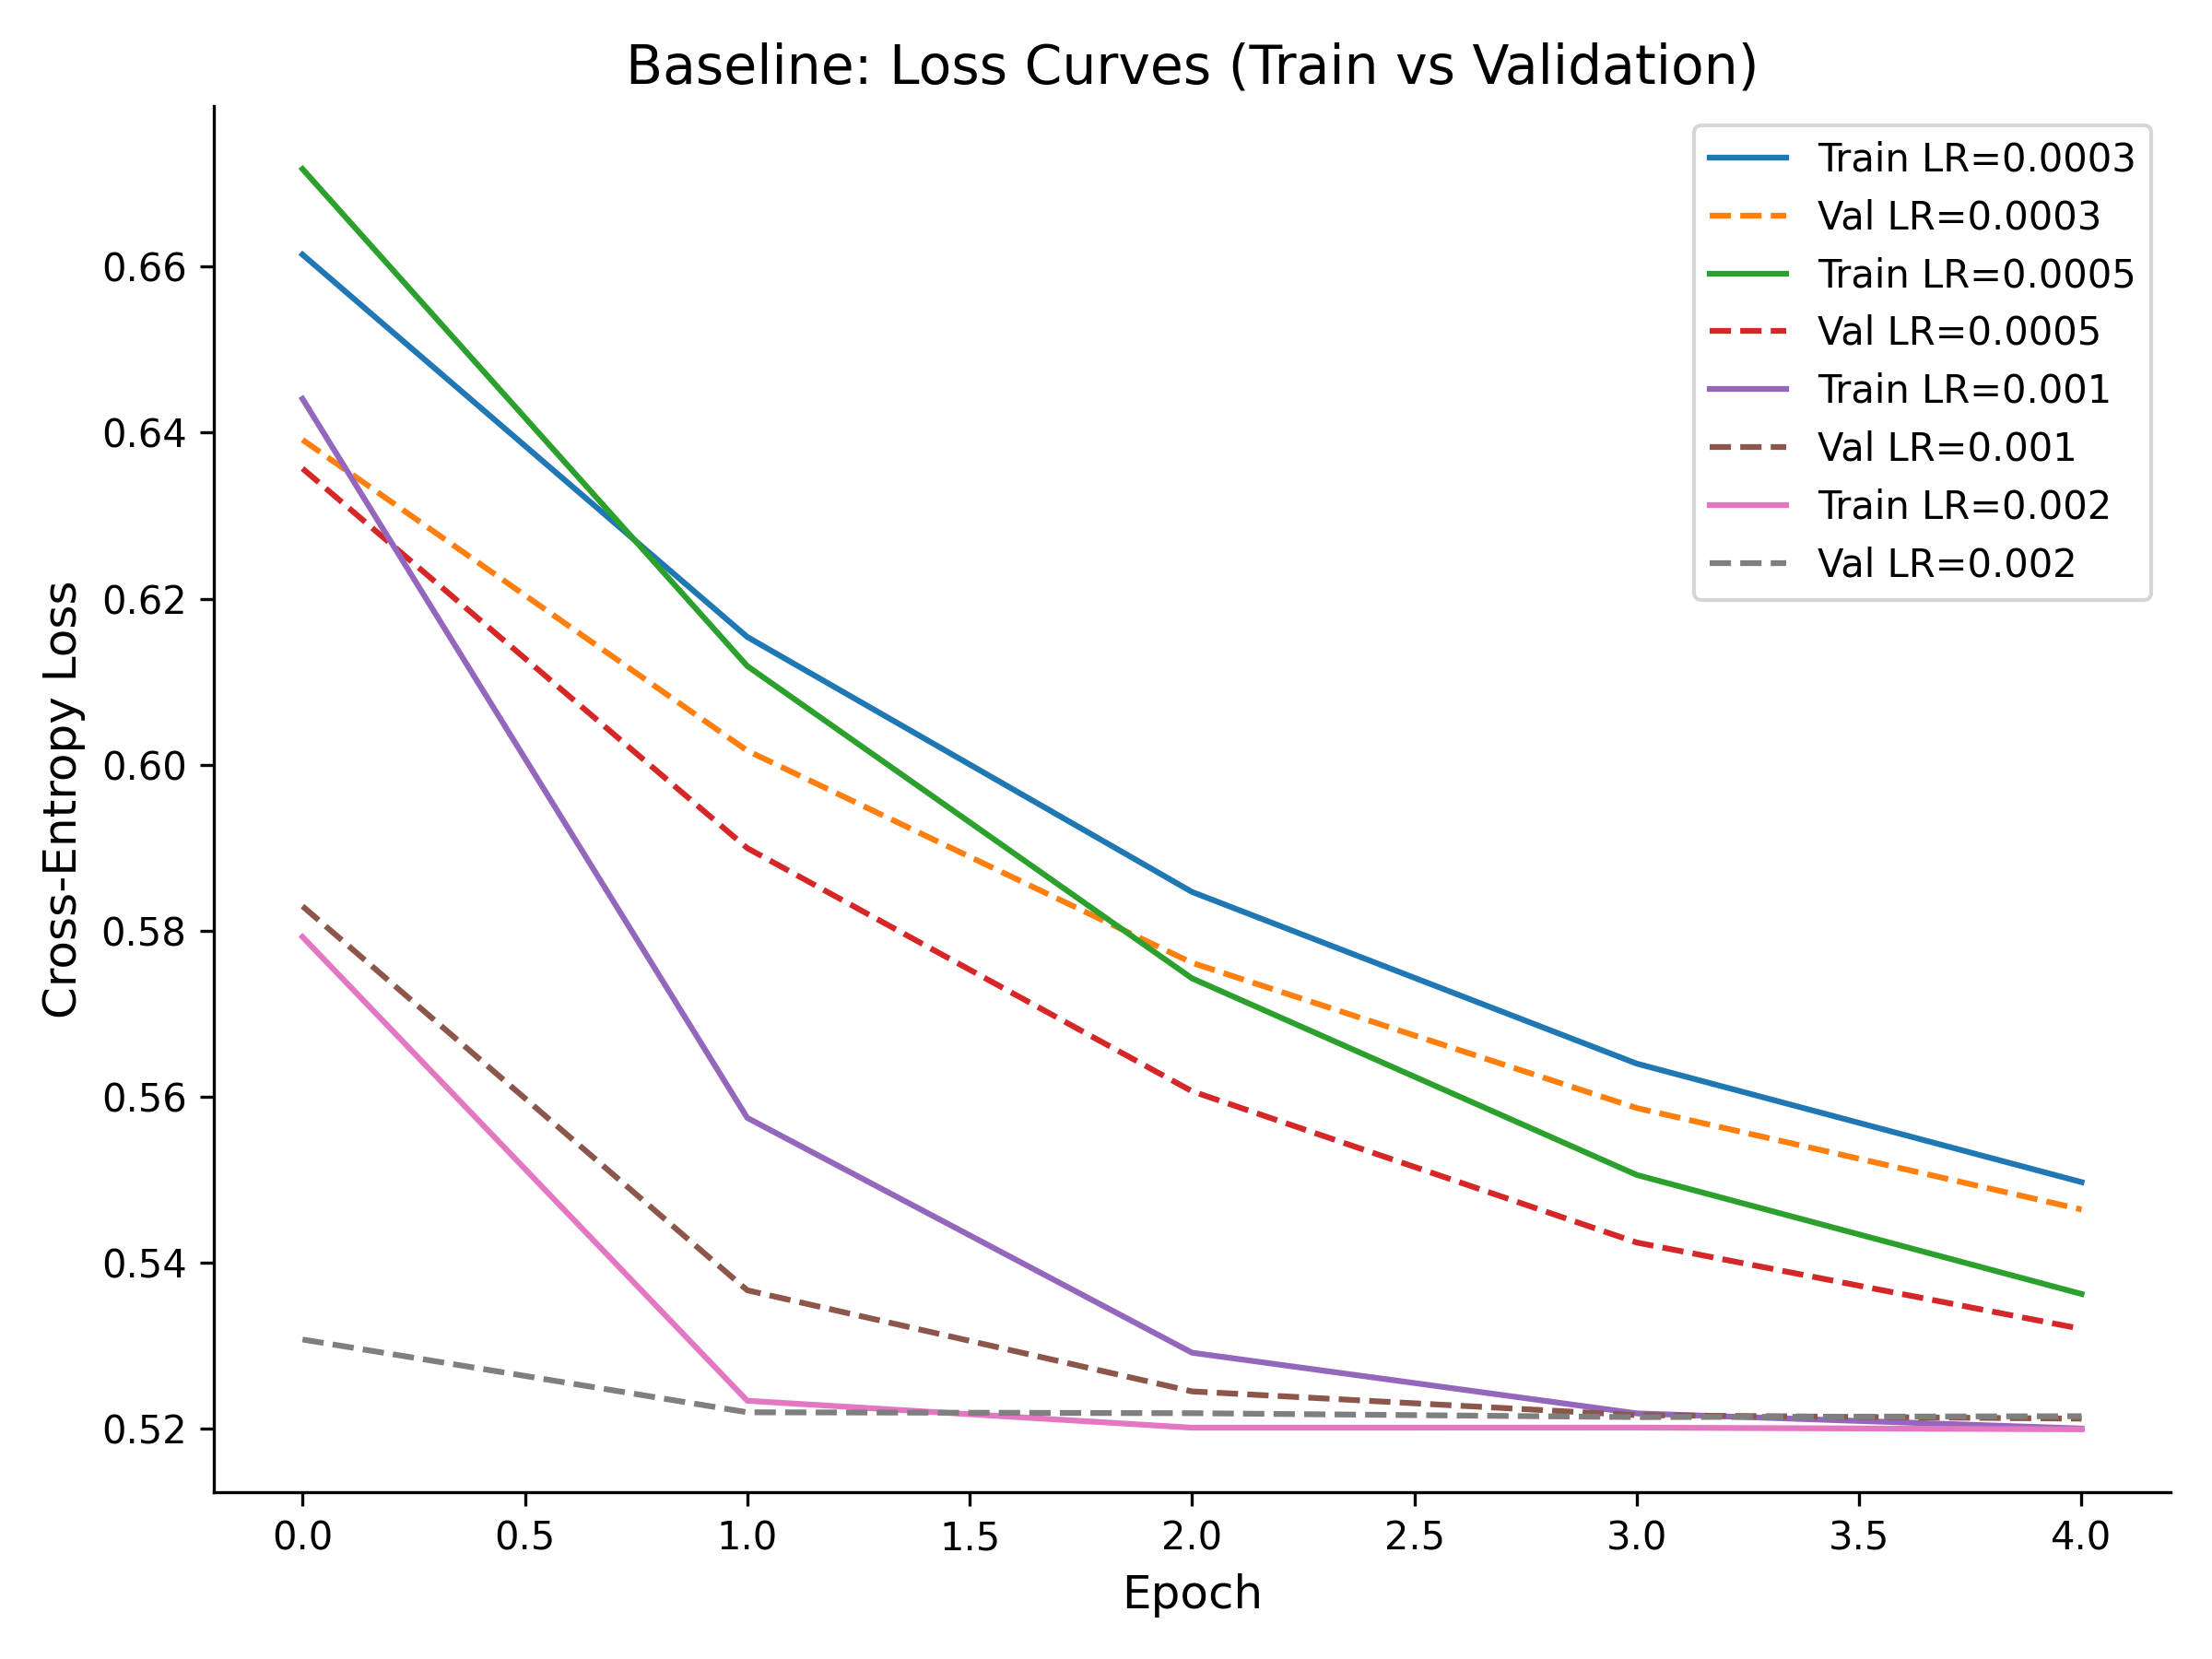
\includegraphics[width=0.45\textwidth]{baseline_loss_curves.png}
\hfill
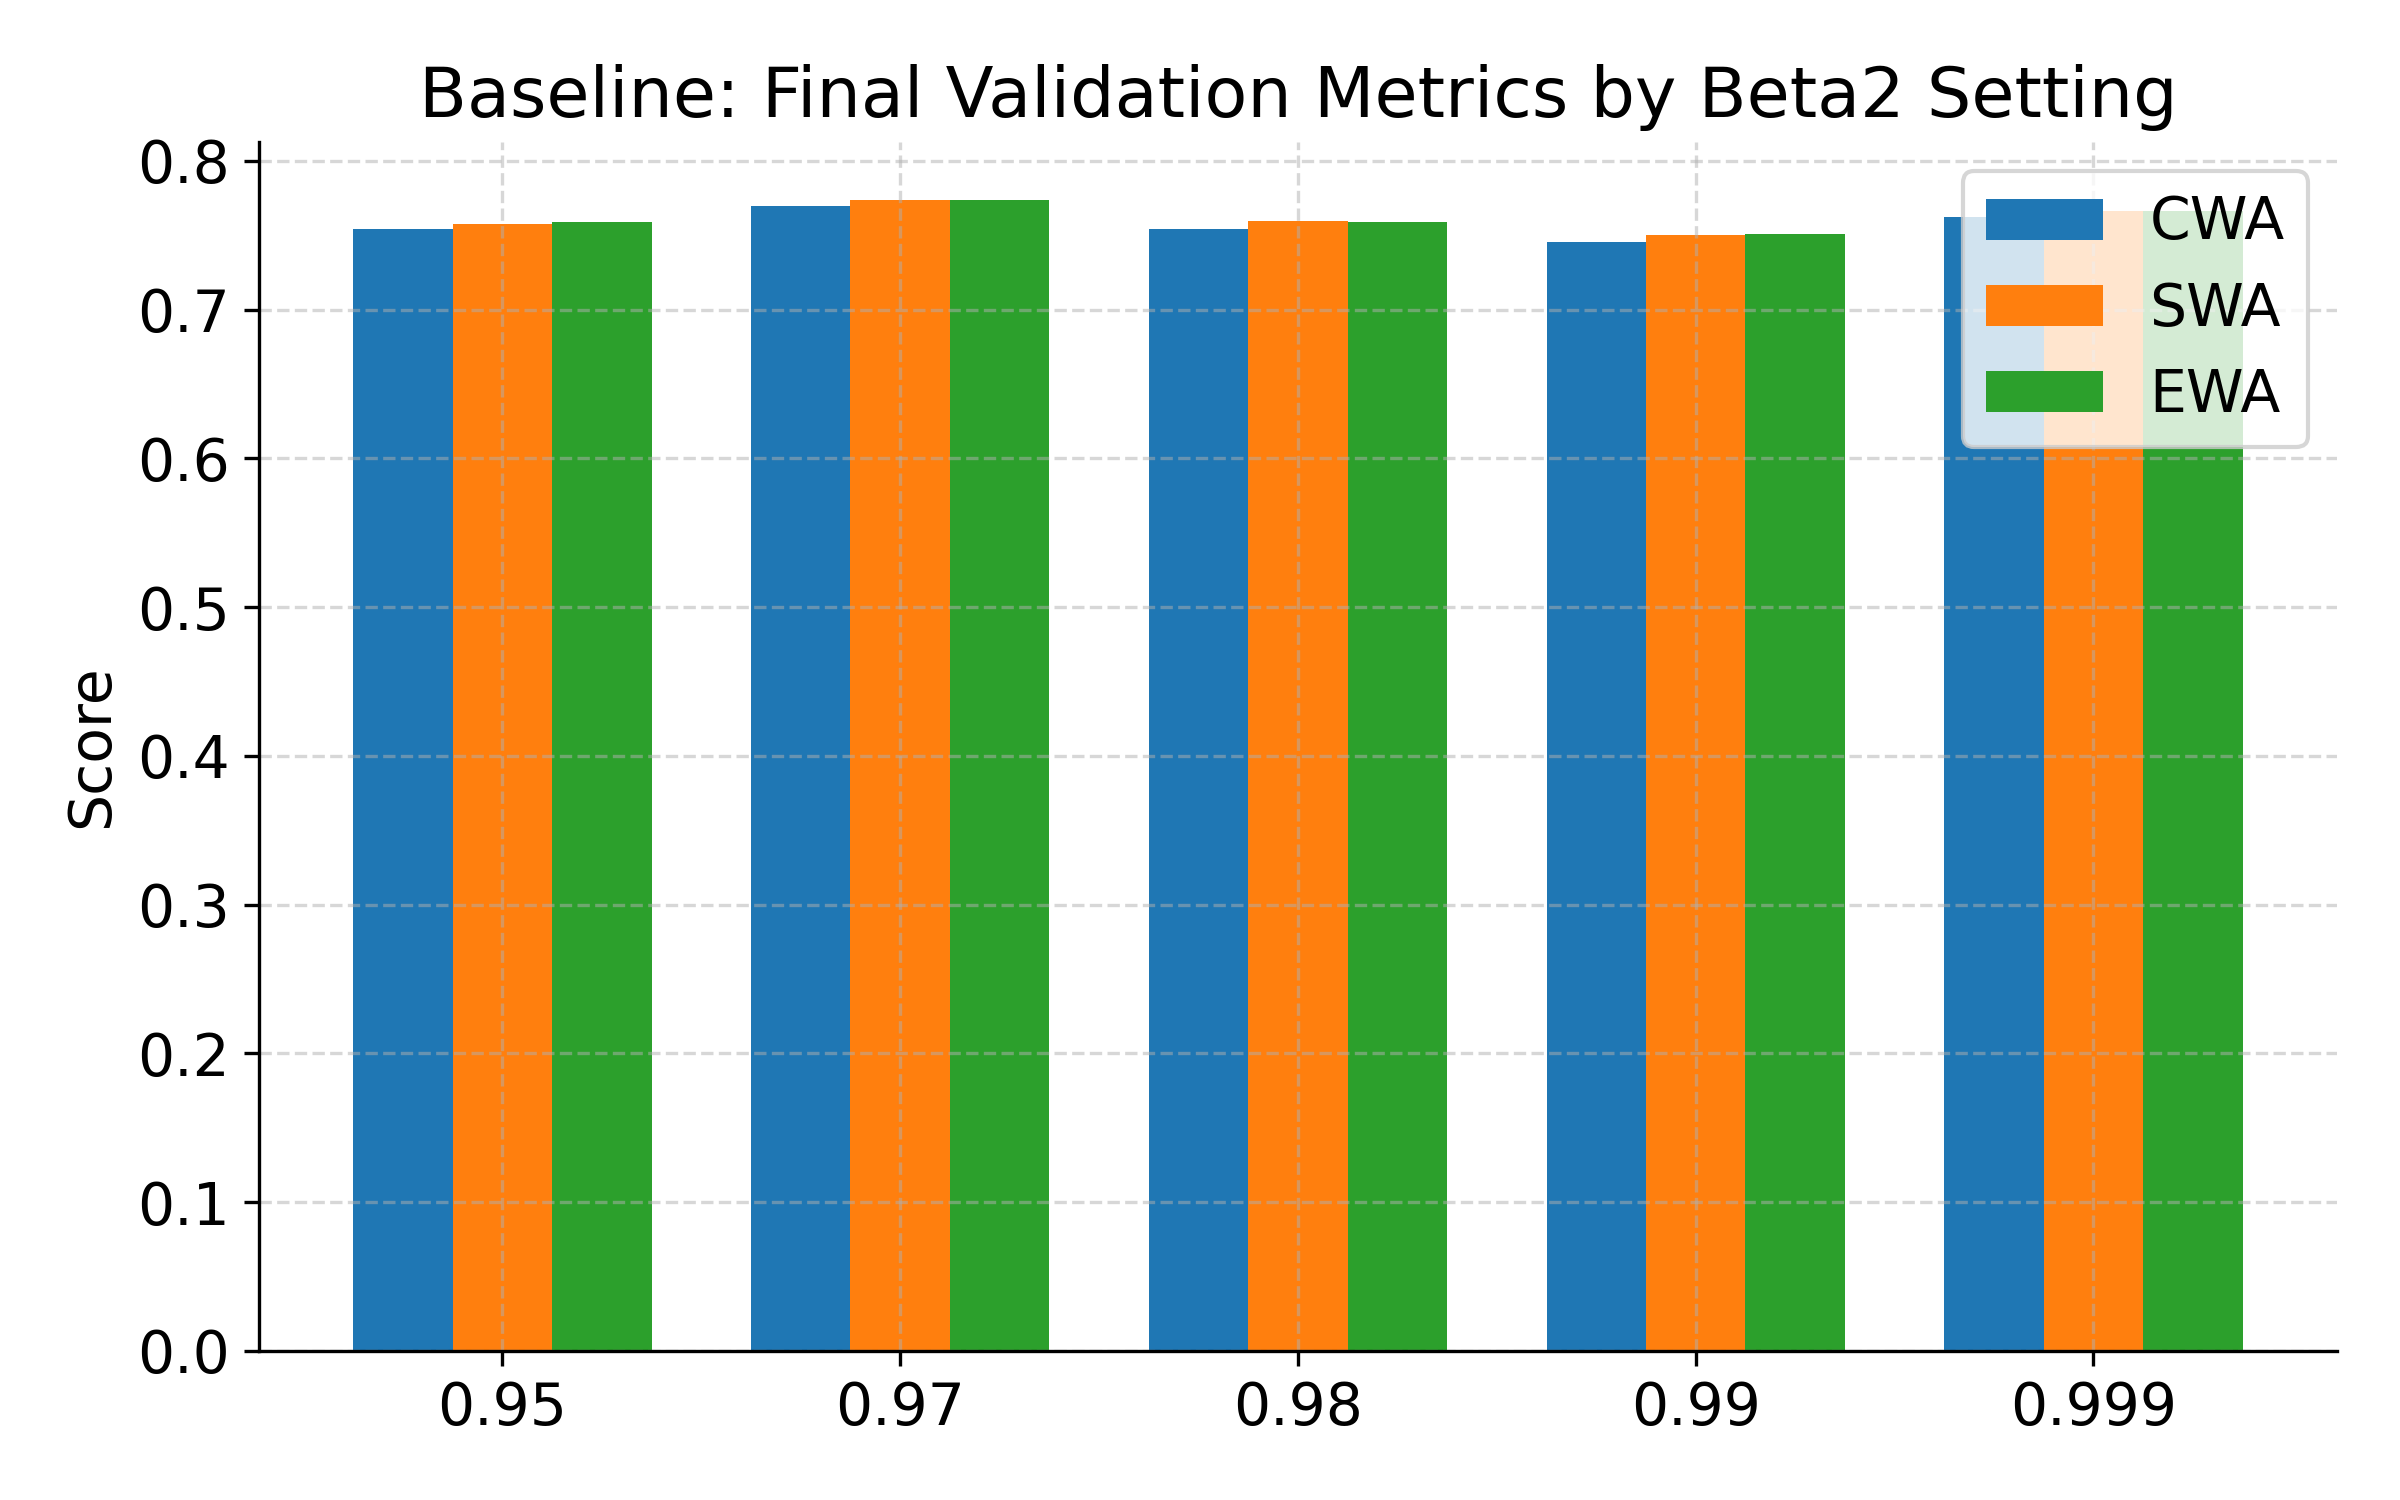
\includegraphics[width=0.45\textwidth]{baseline_final_val_metrics.png}
\caption{\textbf{Baseline results.} (Left) Baseline training and validation losses over time. (Right) Validation metrics under different hyperparameters. Despite apparently smooth convergence, more diverse test sets reveal pitfalls.}
\label{fig:baseline_fig}
\end{figure}

\begin{figure}[t]
\centering
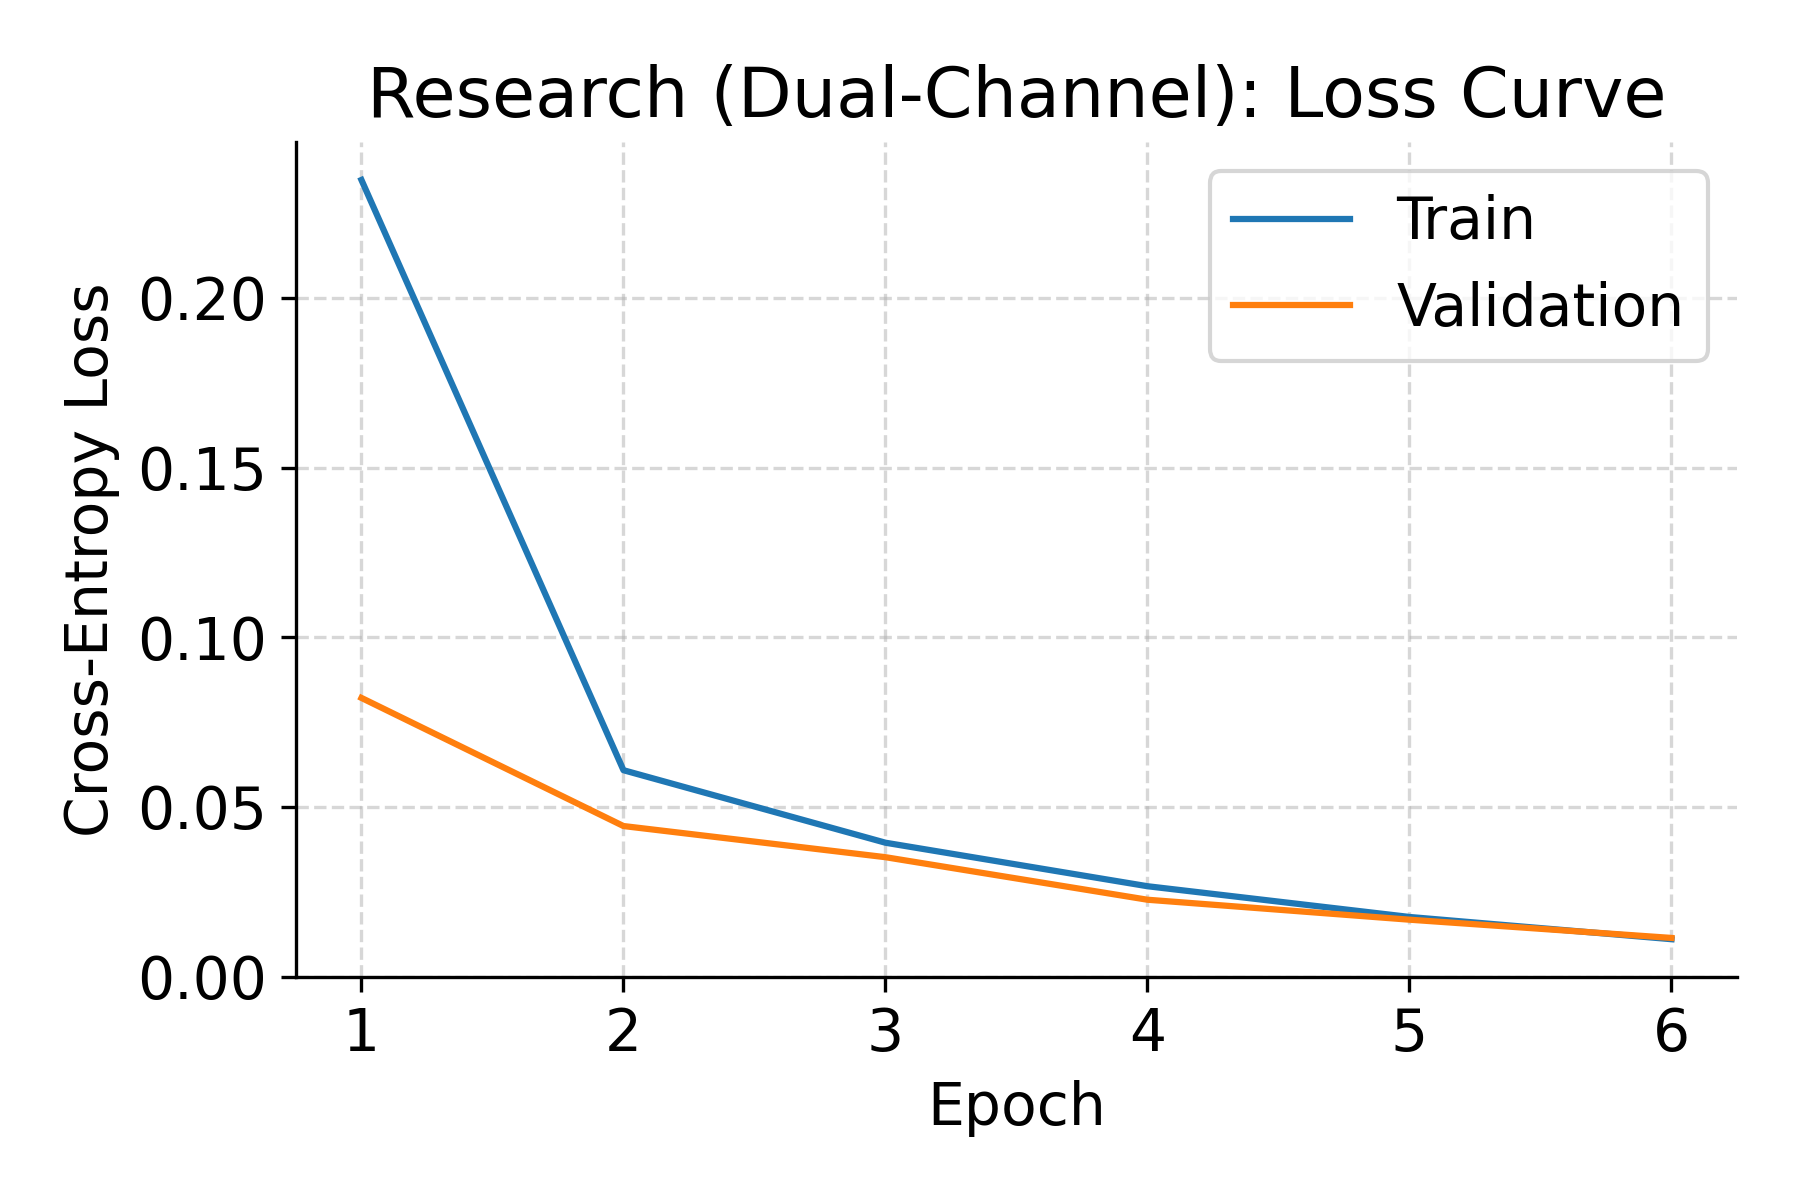
\includegraphics[width=0.45\textwidth]{research_dual_channel_loss_curve.png}
\hfill
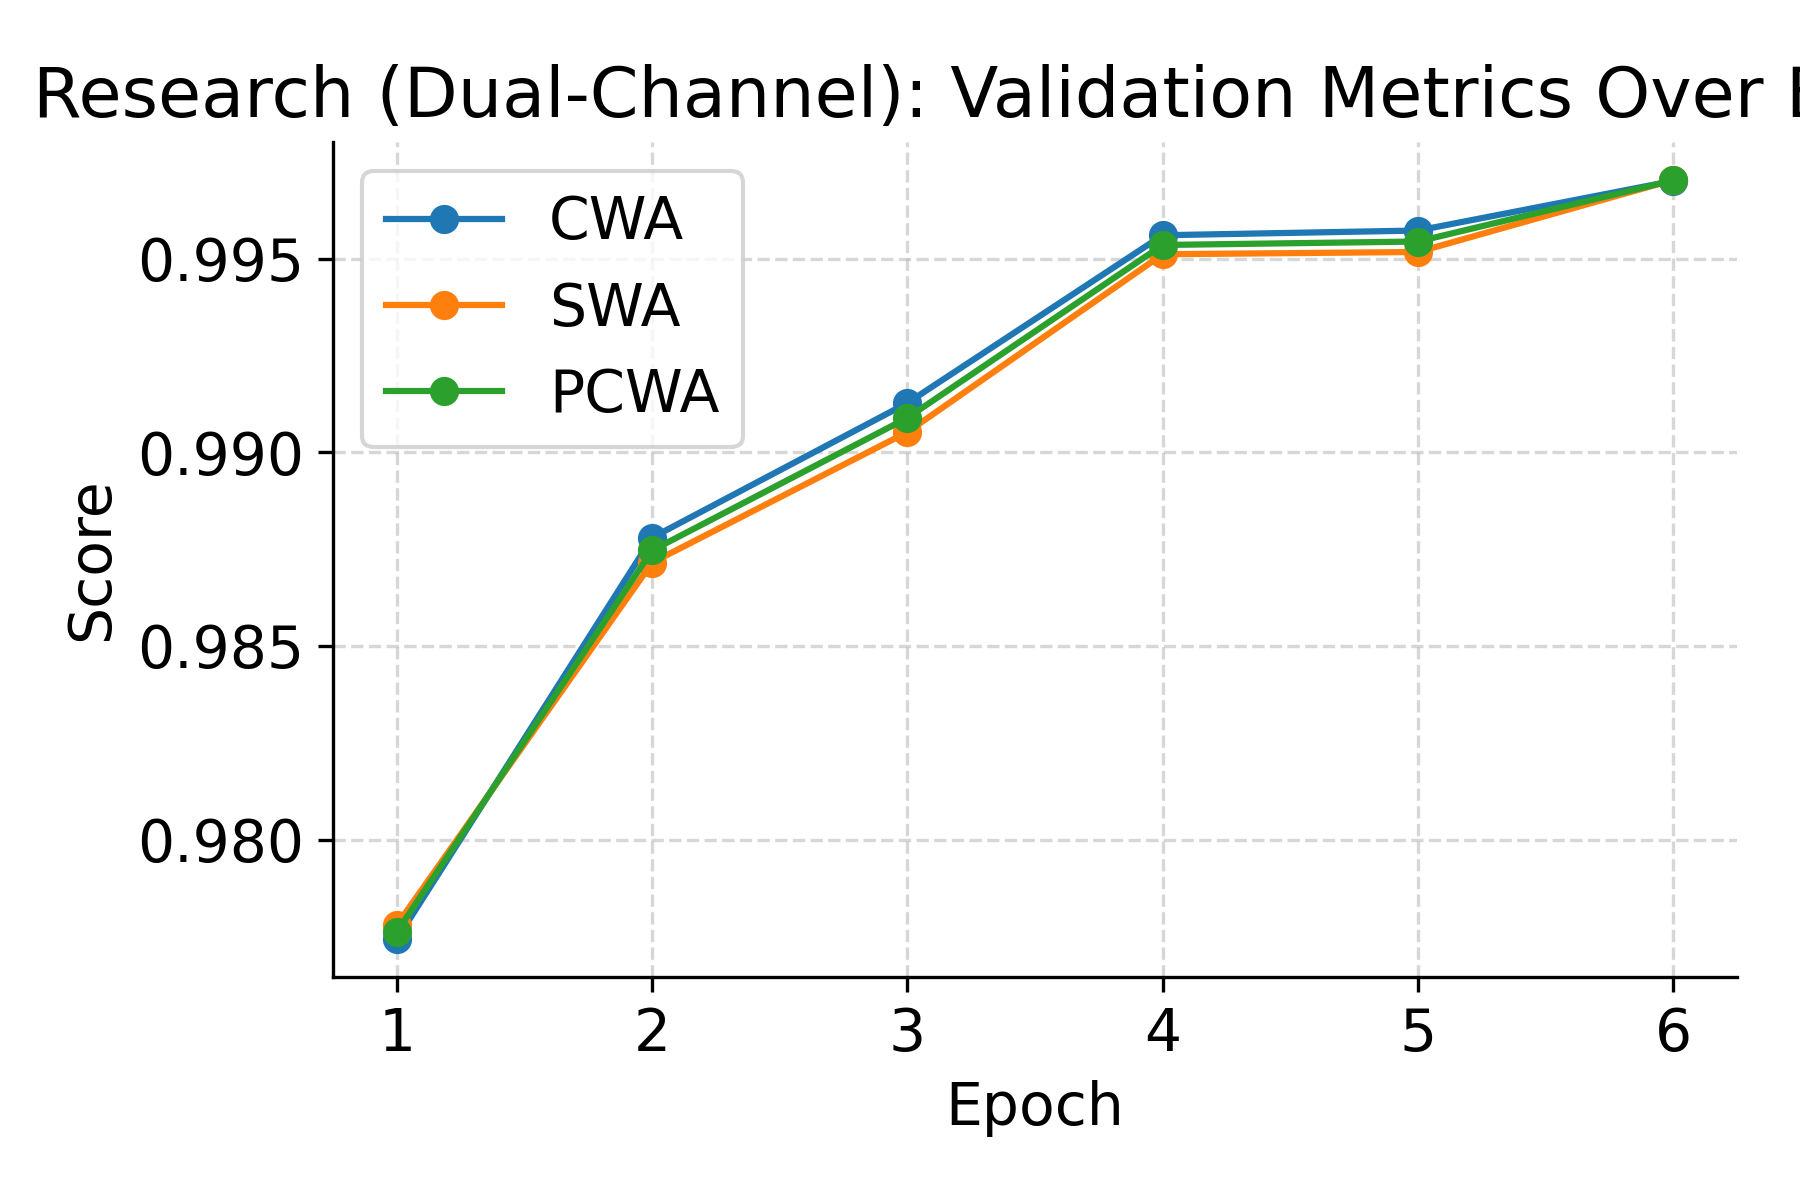
\includegraphics[width=0.45\textwidth]{research_dual_channel_metric_curves.png}
\caption{\textbf{Dual-channel results.} (Left) Loss curves signifying rapid overfitting. (Right) Validation accuracy peaks before dropping, suggesting a potential mismatch between validation distributions and real-world conditions.}
\label{fig:dualchannel}
\end{figure}

\section{Conclusion}
We highlight the discrepancy between validation metrics and genuine generalization in color-shape learning. Our analysis shows how strong validation results can be illusory, prompting practitioners to incorporate broader test scenarios in training pipelines. Future work could explore more robust data augmentation and refined network architectures to avoid these pitfalls.

\appendix
\section{Additional Ablation Studies}
Confusion matrices and ablation experiments detail how removing shape or color inputs impacts performance. See the supplementary figures for visualization of the shape-only model and further breakdowns of training stability. While some ablations partly alleviate overfitting, they still fail to resolve the underlying mismatch between validation and real-world performance.

\bibliographystyle{plain}
\bibliography{references}

\end{document}